\documentclass[00_mcda_tutorial.tex]{subfiles}

\begin{document}
\begin{sidebar*}

\section*{Tutorial 5: Workspace rights management (Enterprise edition)}
\addtocounter{section}{1}
\addcontentsline{toc}{section}{\protect\numberline{}Tutorial 5: workspace rights management}

\subsection*{Subjects covered}
\begin{itemize}
\item Managing other users' rights on your workspaces
\item Changing the owner of a workspace
\end{itemize}

\subsection*{Prerequisites}
\noindent This tutorial assumes some familiarity with the ADDIS/MCDA interface, and also assumes that there is at least one other user registered in the system. 

\subsection*{User rights}
\noindent \faLightbulbO \, In ADDIS/MCDA, a user can have the following rights for a given workspace:
\begin{itemize}
\item Owner: can edit the workspace, and manage who has access.
\item Editor: can edit the workspace.
\item Reader: can view the workspace.
\end{itemize}
By default, users can only view and edit their own workspaces. They can grant access to others explicitly using the rights administration interface.

\subsection*{Getting started}
\leftpointright \, Open your browser and navigate to your MCDA server, and sign in.
\leftpointright \, Create a new workspace for the tutorial by clicking the ‘Create workspace’ button and choosing any example workspace.

\subsection*{List of workspaces}
\noindent \faLightbulbO \, On your personal home page in MCDA, workspaces are sorted by your access rights to them. There are three categories:
\begin{itemize}
\item Workspaces you own
\item Workspaces you can work on (but are not owned by you)
\item Workspaces you can view
\end{itemize}

As an example, see Figure \ref{fig:workspaceList}. If any of the categories is empty, it will not be shown on the page.

{	
	\centering
	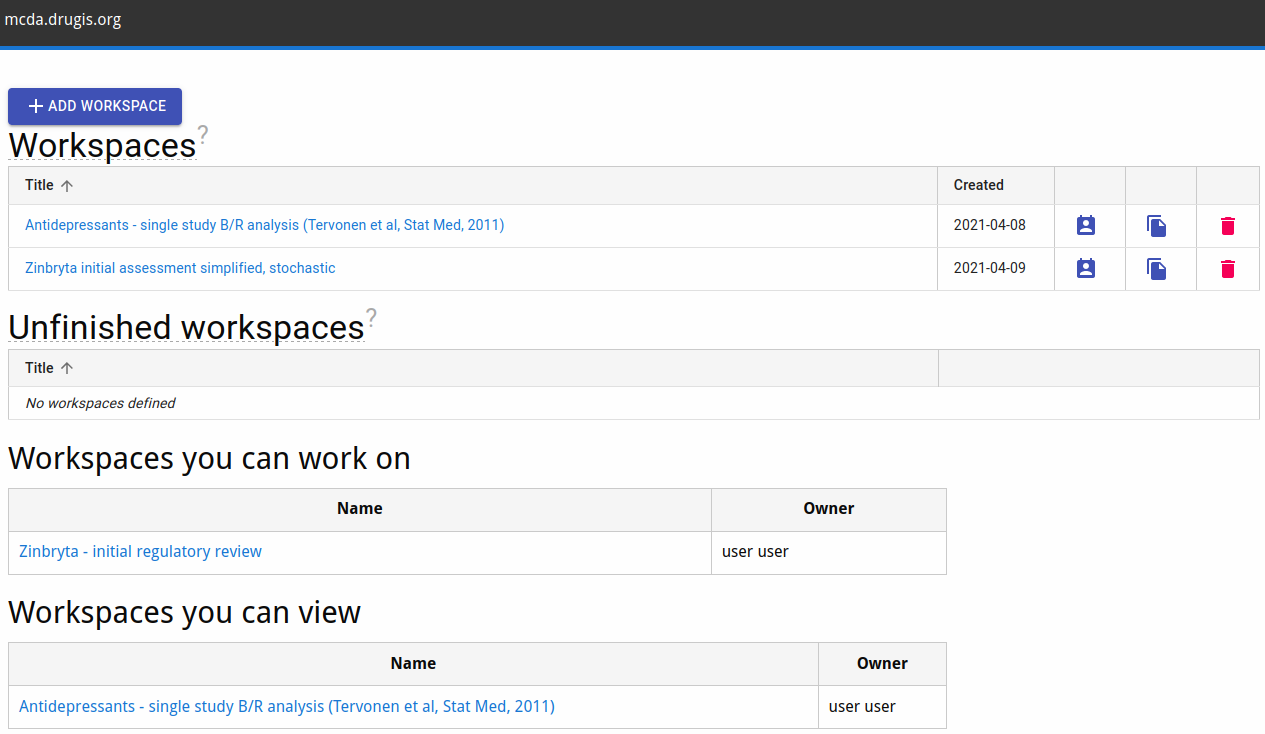
\includegraphics[width=\textwidth]{fig/listWorkspaces.png}
    \captionof{figure}{Workspaces organized in lists.}
	\label{fig:workspaceList}
	\par
}

\subsection*{Manage user rights}
\noindent You will notice that you have several actions available in the list of workspaces that you own.
\leftpointright \, Either from your home page, of from the view of your example workspace, click on the 'Manage user rights' button. This takes you to the user rights management screen. 
You can grant other users Editor or Reader rights using the dropdown menus. Once you are satisfied with your changes, click the 'Save rights' button. 
\noindent \faExclamationTriangle This tutorial cannot predict your environment and tell you who to grant which rights to. Choose a colleague you know, or ask the systems administrator to create an extra testing account.
\noindent \leftpointright \, Besides granting others access, you can also remove rights by clicking the 'Delete' button in the 'Users with rights on this analysis' list. Afterwards, click the 'Save rights' button.

\subsection*{Changing the owner of a workspace}
\noindent \faExclamationTriangle Note that this process is irreversible except by the new owner, or by the administator.
\leftpointright \, Click on the 'Change owner' button. Select a user from the drop down list. This user will be granted ownership of the workspace. Your rights will be set as 'Editor'.
\newline

\end{sidebar*}
\end{document}
